\chapter{OpenBiodiv Linked Open Dataset}
\label{chapter-lod}

We have created a Linked Open Dataset, OpenBiodiv LOD, comprising biodiversity information extracted from Pensoft journals and Plazi Treatment Bank and which was integrated with the GBIF Taxonomic Backbone. As ontology, we use the new \mbox{OpenBiodiv-O} developed by us. We propose to the biodiversity informatics community to use OpenBiodiv LOD as the central point for a biodiversity knowledge graph! OpenBiodiv LOD is an RDF dataset adhering to the principles of Linked Open Data. It is available under \url{http://graph.openbiodiv.net}, which provides a SPARQL endpoint for it.

OpenBiodiv LOD is a synthetic dataset. It does not contain previously unpublished data. Instead it integrates information previously found in academic journals and databases into one dataset. It also contains  extracted, previously unaccessible information from the original datasets in the form of relations. In the next few paragraphs we discuss the sources of information that were combined to from OpenBiodiv LOD and the types of resources that have been extracted, as well as the overall data model. We also discuss the principles of Linked Open Data that tie everything together. The chapter ends with many examples of queries on the dataset and with a technical discussion of how it was generated.

\section{Data Sources}

The data in OpenBiodiv at the time of writing this thesis comes from three major sources: the GBIF Backbone Taxonomy (\cite{gbif_secretariat_gbif_2017-1}), journal articles published by Pensoft, and Plazi Treatment Bank (Fig.~\ref{fig:openbiodiv-sources-simple}).

\begin{figure}
\centering
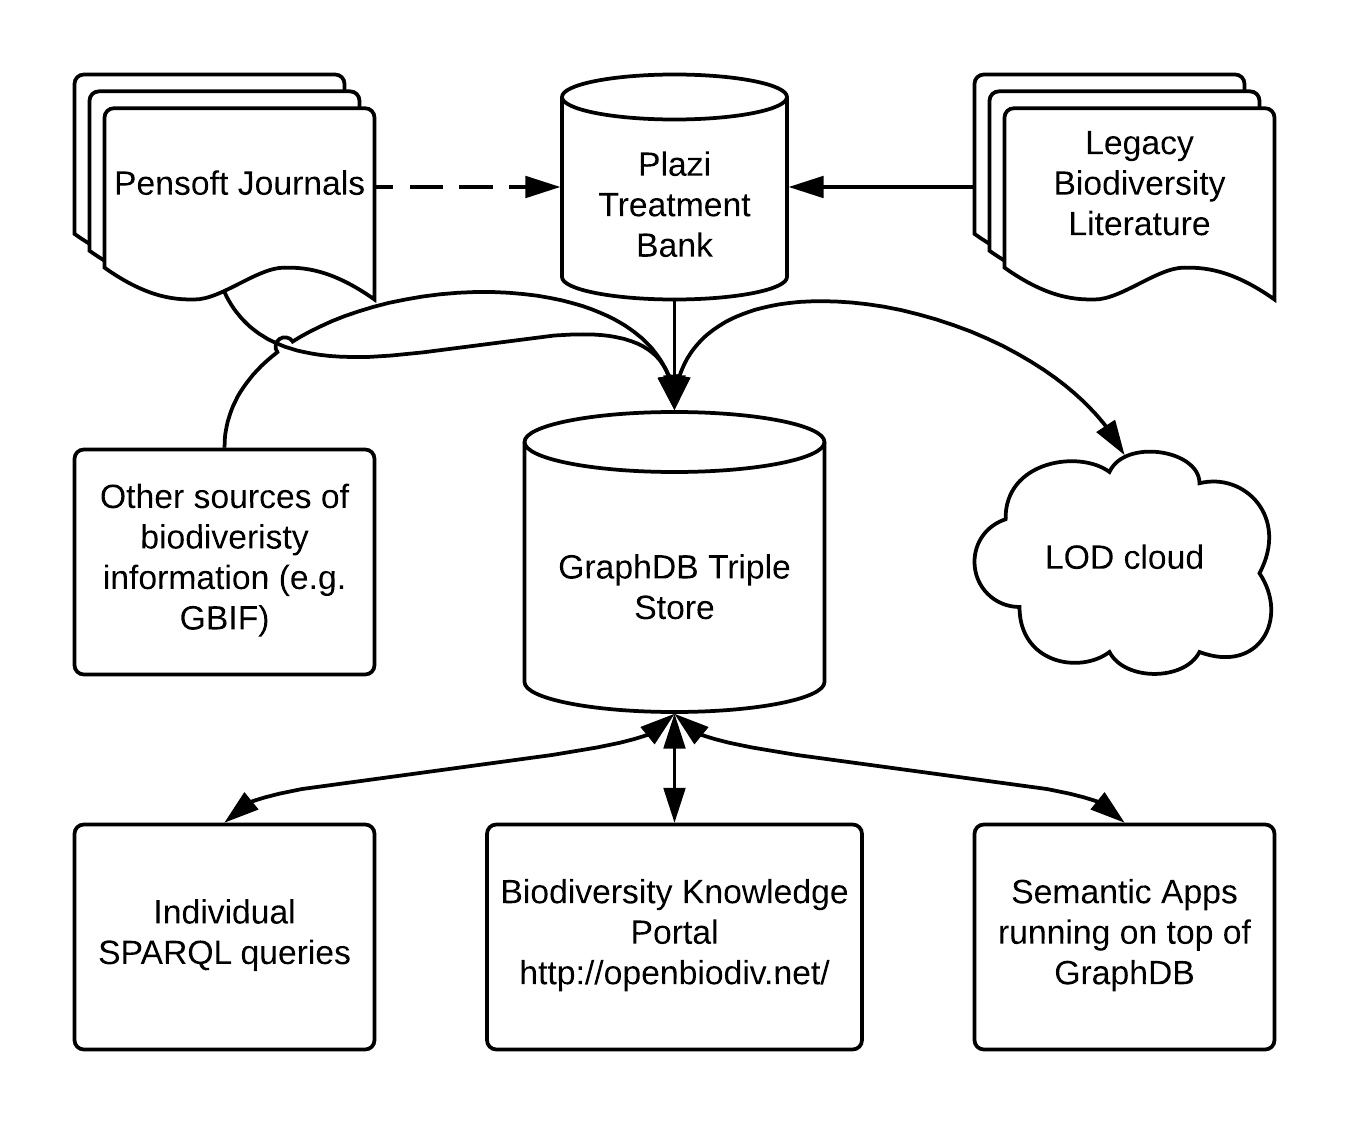
\includegraphics[width=\textwidth]{Figures/openbiodiv-sources-simple}
\decoRule
\caption{A simplified version of the OpenBiodiv architecture presented in Chapter~\ref{chapter-openbiodiv} focusing on the sources of information.}
\label{fig:openbiodiv-sources-simple}
\end{figure}


\subsection{GBIF Backbone Taxonomy}

GBIF is the largest international repository of occurrence data, i.e. data about the presence of an organism of a given taxon at a given place and time. GBIF allows its users to do searches on its occurrence data utilizing a taxonomic hierarchy. For example, it is possible to query the database  for occurrences of organisms belonging to a specific genus: a search for the beetle genus \textit{Harmonia} sec. \cite{gbif_secretariat_gbif_2017-1} on 30 June 2018 returned 575,376 results. This search is possible thanks to the GBIF Backbone Taxonomy also known as Nub (\cite{gbif_secretariat_gbif_2017-1}). Nub is a database organizing taxonomic concepts in a hierarchy covering all names used in occurrence records harvested by GBIF.  It is a single synthetic (algorithmically generated) management classification with the goal of covering all names present in GBIF's datasets. Thus, the GBIF backbone does not represent an expert consensus on how taxa are hierarchically arranged according to evolutionary criteria in Nature.

Keeping in mind this critique, it is evident how the backbone taxonomy allows GBIF to integrate name based information from diverse sources such as Encyclopedia of Life (EOL), Genbank, or the International Union for Conservation of Nature, and provides a facility for taxonomic searching and browsing.

In order to grant the same capabilities to OpenBiodiv, we have imported Nub as instances of {\tt openbiodiv:TaxonomicConcept} according to OpenBiodiv-O. Each GBIF taxonomic concept is linked to an instance of {\tt openbiodiv:ScientificName} and to its parent taxonomic concept via SKOS and RCC-5 (Fig.~\ref{fig:harmonia-halii-visual}). Thus, even though users of OpenBiodiv-LOD have the opportunity of taxonomic search using Nub, we have decoupled scientific names from a single hierarchical representation allowing the future evolution of OpenBiodiv-LOD to incorporate other simultaneous views of taxonomic alignment.

\begin{figure}
\centering
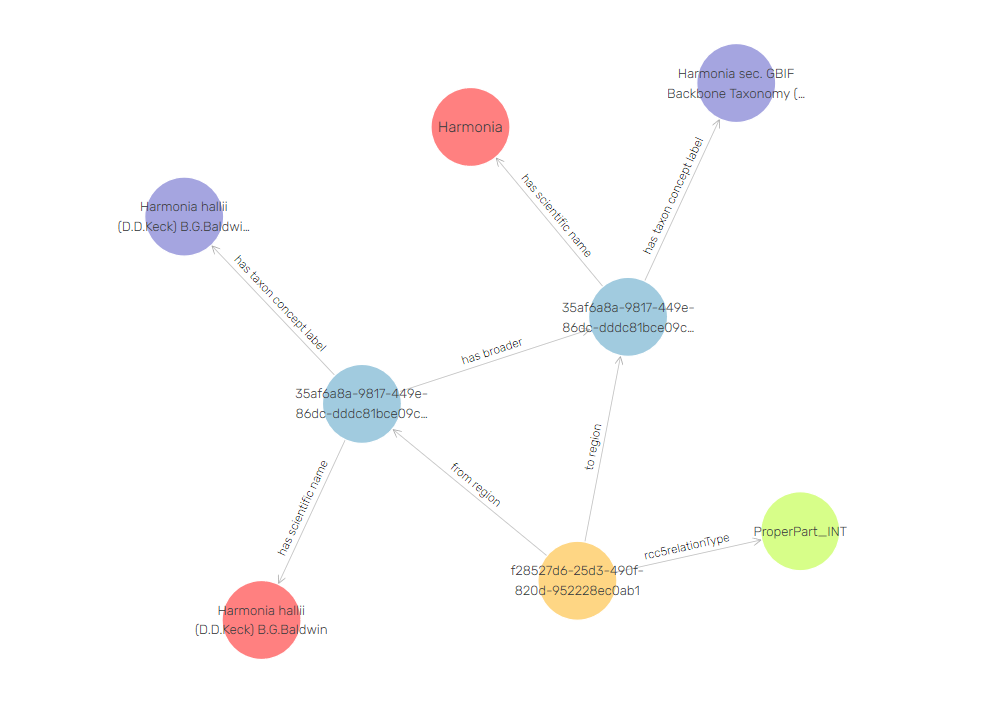
\includegraphics[width=\textwidth]{Figures/harmonia-halii-visgraph}
\decoRule
\caption[Visual graph of \emph{Harmonia halii}]{Illustration of the representation of hierarchical information imported from the GBIF Backbone Taxonomy as two taxonomic concepts, \emph{Harmonia halii} sec. \cite{gbif_secretariat_gbif_2017} and \emph{Harmonia} sec. \cite{gbif_secretariat_gbif_2017}. Each concept has an associated scientific name via \emph{has scientific name}; however, the hierarchical information is not encoded in the names. The hierarchical relationship between \emph{Harmonia halii} sec. \cite{gbif_secretariat_gbif_2017} and \emph{Harmonia} sec. \cite{gbif_secretariat_gbif_2017} is encoded both as SKOS \emph{has broader} and reified via the RCC-5 relationship encoded in {\tt f28527d6-25d3-490f-820d-952228ec0ab1}.}
\label{fig:harmonia-halii-visual}
\end{figure}

Furthermore, as the GBIF backbone taxonomy is updated regularly through an automated process from over 56 sources, future updates may be ingested as different versions into OpenBiodiv-LOD without affecting existing records.

\subsection{Pensoft and Plazi}

All valid articles from the journals published by Pensoft listed in Table~\ref{rdf-pensoft-journals} have been converted to RDF and stored in the biodiversity knowledge graph. Additionally, all valid taxonomic treatments from Plazi Treatment Bank have been converted to RDF and stored in the graph as well. Furthermore, the RDF-ization procedure is triggered automatically on a weekly basis and thus the semantic database is always updated with the newest articles published by Pensoft and newest taxonomic treatments extracted by Plazi. The RDF-ization is made possible by the fact that all Pensoft journals are published as XML according to TaxPub, an extension of the NLM/NCBI journal publishing DTD for taxonomic description (\cite{catapano_taxpub:_2010}) and, similarly, all Plazi treatments follow the TaxonX XML Schema (\cite{penev_xml_2011}). Thus, the RDF-ization pipeline does not require a natural language processing step, as a considerable amount of information is marked-up at the time of publication. We have given an example of how a taxonomic name usage is marked up in a TaxPub article in Listing~\ref{listing:tnu}. The datatypes that have been marked up in TaxPub and TaxonX and whose entities are converted to RDF are listed in Table~\ref{datatypes-taxpub-taxonx}. Note that the marked-up datatypes do not correspond 1-to-1 to the RDF entities that have been created in the graph as TaxPub, TaxonX, and OpenBiodiv-O take slightly different approaches to modeling the biodiversity world. OpenBiodiv-O takes the most granular approach. For example, each taxonomic name usage in a Pensoft article results in a corresponding {\tt openbiodiv:TaxonomicNameUsage} resource and a link to the {\tt openbiodiv:ScientificName} resource that the taxonomic name usage mentions (Fig.~\ref{fig:tnu-vis}).

\begin{lstlisting}[language=XML,
caption=Taxonomic name usage of the name \emph{P. emarginaticeps} in Taxpub. Name parts are tagged with {\tt tp:taxon-name-part} and the expansion of abbreviations (regularization) is marked up with the attribute {\tt reg},
label=listing:tnu, basicstyle=\ttfamily\tiny]
<tp:taxon-name>
  <tp:taxon-name-part taxon-name-part-type="genus" reg="Pristaulacus">
    P.
  </tp:taxon-name-part>
  <tp:taxon-name-part taxon-name-part-type="species" reg="emarginaticeps">
    emarginaticeps
  </tp:taxon-name-part>
  <tp:taxon-name-part taxon-name-part-type="authority">
    Turner 1922
  </tp:taxon-name-part>
</tp:taxon-name> 
\end{lstlisting}

\begin{table}[h!]
\caption{RDF-ized biodiversity journals published by Pensoft.}
      \begin{tabular}{ccc}
        \hline
          Journal Name             & Submission Style & Number of Articles\\  \hline
          ZooKeys                 & Word document & 3829\\
          PhytoKeys               & Word document & 537\\
          MycoKeys                & Word document & 127\\
          Biodiversity Data Journal & Web based (ARPHA) & 490\\
          Journal of Orthoptera Research & Word document & 32
      \end{tabular}
      \label{rdf-pensoft-journals}
\end{table}

\begin{table}[h!]
\caption{Datatypes marked up in TaxPub and TaxonX articles and the corresponding RDF types of the generated RDF resources. The TaxPub and TaxonX columns contain boolean values indicating whether the information about the datatype is retrieved from files encoded in the corresponding schema.}
      \begin{tabular}{cccc}
        \hline
          Datatype             & TaxPub & TaxonX & RDF Type\\  \hline
          Article metadata     & T & T & {\tt fabio:JournalArticle} and related\\
          Keyword group        & T & F & {\tt openbiodiv:KeywordGroup} \\
          Abstract             & T & T & {\tt sro:Abstract}\\
          Title                & T & F & {\tt doco:Title} \\
          Author               & T & T & {\tt foaf:Person} \\
          Introduction section & T & F & {\tt deo:Introduction}\\
          Discussion section   & T & T & {\tt orb:Discussion}\\
          Treatment section    & T & T & {\tt openbiodiv:Treatment}\\
          Nomenclature section & T & T & {\tt openbiodiv:NomenclatureSection}\\
          Materials examined   & T & T & {\tt openbiodiv:MaterialsExamined}\\
          Diagnosis section    & T & T & {\tt openbiodiv:DiagnosisSection} \\
          Distribution section & T & T & {\tt openbiodiv:DistributionSection}\\
          Taxonomic key        & T & T & {\tt openbiodiv:TaxonomicKey}\\
          Figure               & T & T & {\tt doco:Figure}\\
          Taxonomic name usage & T & T & {\tt openbiodiv:TaxonomicNameUsage}
      \end{tabular}
      \label{datatypes-taxpub-taxonx}
\end{table}

\begin{figure}
\centering
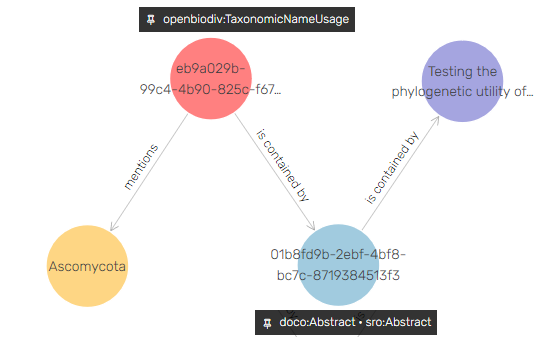
\includegraphics[width=\textwidth]{Figures/tnu-vis}
\decoRule
\caption[Visual graph of a taxonomic name usage]{The taxonomic name usage ({\tt openbiodiv:eb9a029b-99c4-4b90-825c-f670fb88900d}) is linked to the scientific name it mentions, \emph{Ascomycota} and to the part of the article (abstract) that it is contained in.}
\label{fig:tnu-vis}
\end{figure}

\section{Linked Open Data}

Linked Open Data (LOD, \cite{heath_linked_2011}) is a concept of the Semantic Web (\cite{berners-lee_semantic_2001}) applied to ensure that data published on the Web is reusable, discoverable and most importantly to ensure that pieces of data published by different entities can work together. The principles of LOD are the following (\cite{heath_linked_2011})

\begin{enumerate}
\item{Use URIs as names for things.}
\item{Use HTTP URIs so people can lookup these things.}
\item{When someone looks up a URI, provide useful information, using the standards (RDF, SPARQL).}
\item{Include links to other URIs so they can discover more things.}
\end{enumerate}

We have followed these guidelines when creating the OpenBiodiv LOD. We will now discuss each of these points separately.

\subsection{Usage of URIs as resource identifiers}

Every instance in OpenBiodiv LOD is uniquely identifiable by a HTTP URI of the following form: \url{http://openbiodiv.net/uuid-(suffix)}. All instance identifiers in OpenBiodiv LOD follow this schema. The optional suffix field is assigned only to resources extracted from GBIF.

\paragraph{Identfiers for Pensoft and Plazi.} During the RDF-ization of the sources Pensoft and Plazi, when a new concept is discovered (e.g. a person, a scientific name, etc.) a UUID is generated. Then the resource is always referred to in the database by this UUID in the OpenBiodiv namespace, \url{http://openbiodiv.net/}. Pensoft and Plazi furthermore share the UUID part of the identifier in the semi-structured representation of treatments. For example, Lyubomir Penev is a resource identified by \url{http://openbiodiv.net/7a247614-878b-4d01-ab97-bf5fc608dc86}.

\paragraph{Identifiers for GBIF taxonomic concepts.} GBIF offers its taxonomic backbone as a big DarwinCore (\cite{wieczorek_darwin_2012}) tab separated file (TSV). Each row in the TSV corresponds to a taxonomic concept published by GBIF. GBIF does not offer a globally unique ID of its concepts, but only a local ID (e.g. $4239$ is the GBIF ID of concept of Curculionidae sec \cite{gbif_secretariat_gbif_2017}). This is why, we generated a UUID (e.g. for the example \url{35af6a8a-9817-449e-86dc-dddc81bce09c-4239}) for each row of data table published from GBIF. However, each taxonomic concept is linked to a taxonomic name and to a taxonomic concept label (see Chapter~\ref{chapter-ontology}. It was impractical for programmatic reasons to generate a new UUID for these linked entities. This is why their unique identifiers are suffixed. We use the suffix \url{-ScientificName} to denote scientific names and \url{-TCL} to denote taxonomic concept labels.

In our example we have respectively\\\url{http://openbiodiv.net/35af6a8a-9817-449e-86dc-dddc81bce09c-4239-ScientificName}\\and \url{http://openbiodiv.net/35af6a8a-9817-449e-86dc-dddc81bce09c-4239-TCL}.

\subsection{Usage of HTTP URIs and dereferencing}

As per the Linked Data Principles, we use dereferenceable HTTP URIs for our resources. For example, if a web-browser opens\\\url{http://openbiodiv.net/35af6a8a-9817-449e-86dc-dddc81bce09c-4239-ScientificName} a web-page is displayed (Fig.~\ref{fig:portal-name-visualization}) providing useful information for the name such as where it used and other names are related to it. Also it is possible to request OpenBiodiv resources via Curl with the header {\tt Content-Type: application/rdf+xml} and an RDF representation of the resources is returned.

\begin{figure}
\centering
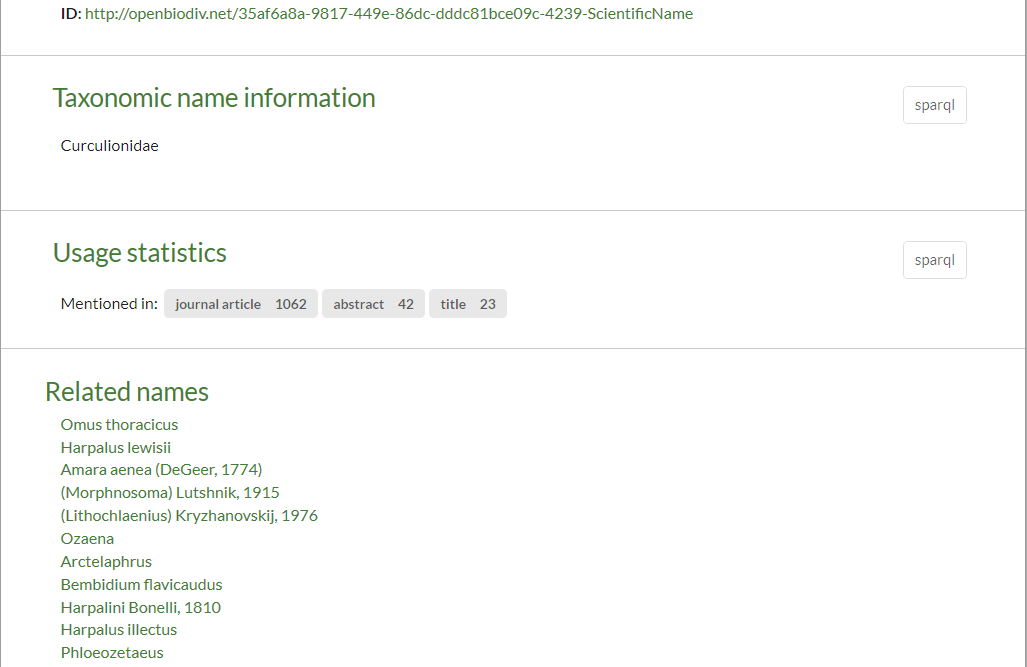
\includegraphics[width=\textwidth]{Figures/portal-name-visualization}
\decoRule
\caption{Visualization.}
\label{fig:portal-name-visualization}
\end{figure}

\subsection{Linking to other resources}

First, all resources in OpenBiodiv form a graph (there are no disconnected parts). The data model is discussed in the next section. Second taxonomic names are linked to external databases via \url{dwc:taxonID}. These are strings containing GBIF ID's, ZooBank ID's, LSID's, etc. Unfortunately as HTTP URI's have not gained popularity in the biodiversity informatics community, the only true resource-id-to-resource-id links are within OpenBiodiv itself. However, we hope that the introduction of OpenBiodiv LOD contributes to the amelioration of this situation.

\section{Data Model}

When creating the RDF graph we have conformed to the OpenBiodiv Ontology described in Chapter~\ref{chapter-ontology} and well-established community ontologies (Fig.~\ref{fig:community-ontologies}). In particular, (1) we use the Semantic Publishing and Referencing Ontologies (SPAR, \cite{peroni_semantic_2014}) to model entities from publishing such as Journal, Article, Section, Figure, Table, and so on; and (2) we use the DarwinCore (DwC, \cite{wieczorek_darwin_2012}) community standard and its extension, the Darwin-SW (\cite{baskauf_darwin-sw:_2016}) ontology, to model entities the biodiversity domain.

\begin{figure}
\centering
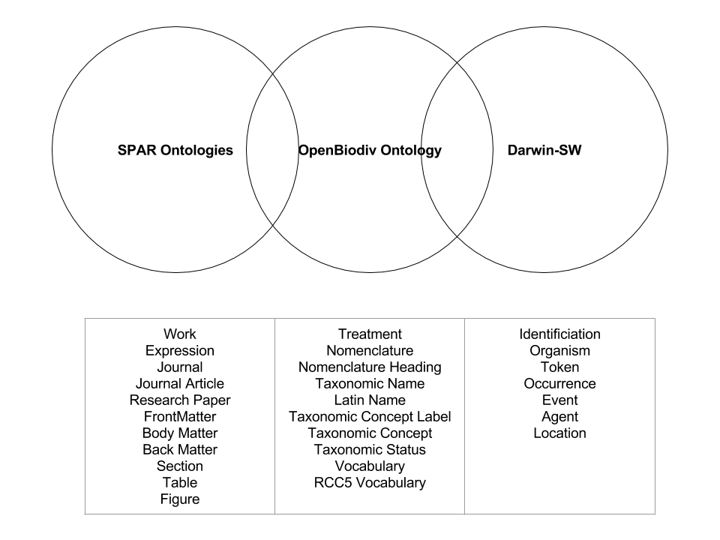
\includegraphics[width=\textwidth]{Figures/community-ontologies}
\decoRule
\caption[Overlap of OpenBiodiv-O with Community Ontologies]{OpenBiodiv-O is an ontology that links the publishing domain with the biodiversity domain. Major resource types covered by each of the ontology families are given in the box below the Venn diagram. Important resources from the publishing domain are listed in the leftmost column and from biodiversity informatics in the rightmost column. The middle one covers important OpenBiodiv-O resources.}
\label{fig:community-ontologies}
\end{figure}

SPAR provides facilities to deal with the dichotomy between the abstract representation of knowledge through the class Work and its concrete representation through the class Expression. For example, a {\tt fabio:JournalArticle} can be the realization of a {\tt fabio:ResearchPaper}. On the other hand, the DwC community standard gives a standard way to express properties from taxonomy and biodiversity science and its extension Darwin-SW a way to reify elements of an occurrence instance such as Identification, Organism, Token, and so on. A caveat: the current version of OpenBiodiv-LOD does not store yet occurrence information but all necessary infrastructure is in place to include them in the next release.

\section{Examples SPARQL queries}

As SPAR, DwC, and OpenBiodiv-O have already been explained elsewhere, we shall illustrate the data model by issuing sample SPARQL queries illuminating aspects of it.

\subsection{Simple queries}

\subsubsection{Query for author} Authors are instances of {\tt foaf:Person} (except in the rare institutional case, in which case they would be {\tt foaf:Agent}'s) and are \emph{creator}-s of Works that have an Expression. The SPARQL query in Listing~\ref{listing:prolific_author} answers the question of which author has been on the author list of the most articles. Note that the results may change as new articles are added to the graph.

\lstinputlisting[language=SPARQL,
caption=Most prolific author SPARQL query.,
label=listing:prolific_author, basicstyle=\ttfamily\tiny]
{Listings/prolific-author.SPARQL.txt}

\subsubsection{Query for scientific name}

Latin names are stored in the system as {\tt :ScientificName}'s are are \emph{mention}-ed by taxonomic name usages.

Listing~\ref{listing:mentioned_name} orders scientific names of any rank by the number of unique mentions that they have in articles. It is possible to narrow down the solution to binomial names (species names) by adding the {\tt dwciri:taxonRank} property as shown in Listing~\ref{listing:mentioned_species_name}. In order to see the different ranks that scientific names are assigned to in OpenBiodiv you can use the query in Listing~\ref{listing:ranks}. It is also possible, for example, to determine the most mentioned scientific name by the number of articles it is mentioned in (Listing~\ref{listing:mentioned_name_articles}).

\lstinputlisting[language=SPARQL,
caption=Most mentioned scientific name.,
label=listing:mentioned_name, basicstyle=\ttfamily\tiny]{Listings/name-mentions.SPARQL.txt}

\lstinputlisting[language=SPARQL,
caption=Most mentioned species name.,
label=listing:mentioned_species_name, basicstyle=\ttfamily\tiny]{Listings/species-name-mentions.SPARQL.txt}

\lstinputlisting[language=SPARQL,
caption=What are the available taxonomic ranks?,
label=listing:ranks, basicstyle=\ttfamily\tiny]{Listings/ranks.SPARQL.txt}

\lstinputlisting[language=SPARQL,
caption=Most mentioned species name by number of articles that mention it.,
label=listing:mentioned_name_articles, basicstyle=\ttfamily\tiny]
{Listings/species-name-mentions-by-articles.SPARQL.txt}

\subsubsection{Query the article structure} A unique feature of OpenBiodiv LOD is that articles are broken down into their components (see e.g. Table~\ref{datatypes-taxpub-taxonx} later in this Chapter) and mentions (e.g. taxonomic name usages) connect to the specific part of the article and not just to the article in general.

Combining this feature with queries from the previous paragraph, we can, for example, look for the most mentioned scientific name in a figure (Listing~\ref{listing:mentioned_name_figures}). The only difference in this query is that we have replaced the type of {\tt ?a} with {\tt doco:Figure}. 

\lstinputlisting[language=SPARQL,
caption=Most mentioned scientific name in figures,
label=listing:mentioned_name_figures, basicstyle=\ttfamily\tiny]
{Listings/name-mentions-by-figure.SPARQL.txt}

We can look, for example, for the figures present in a particular article (Listing~\ref{listing:figures_article})

\lstinputlisting[language=SPARQL,
caption=Figures of a given article., label=listing:figures_article, basicstyle=\ttfamily\tiny]
{Listings/figures-of-article.SPARQL.txt}

\subsubsection{Query for taxonomic concepts}

A key feature of OpenBiodiv-O is that it allows for the separation of taxonomic concepts from scientific names. Scientific names are linked both to the components of an article that mentions them and to taxonomic concepts. To illustrate this, we can create a query uniting information from concepts from the GBIF Backbone Taxonomy (next subsection) with semantics coming from the article structure. The query in Listing~\ref{listing:new_curcu} locates the beetle family Curculionidae sec. \cite{gbif_secretariat_gbif_2017} in the system, and looks for new taxa ({\tt :TaxonomicDiscovery}) that have been associated with one of its genera.

\lstinputlisting[language=SPARQL,
caption=Taxonomic discoveries in the weevils., label=listing:new_curcu, basicstyle=\ttfamily\tiny]
{Listings/new-curculionidae.SPARQL.txt}

\subsubsection{Fuzzy Queries via Lucene}

The SPARQL endpoint of OpenBiodiv LOD supports fuzzy matching via a Lucene connector (\cite{ontotext_graphdb_2018}). In taxonomy, this can be a very useful as due to multiplicity of taxonomic names and the complexities of Latin grammar, one often does not remember the correct spelling of a name. This can lead to no matches in an exact search even though the system may contain information about that name.

Lucene queries at the OpenBiodiv workbench are made in SPARQL. In order to carry out a Lucene query, one matches the following graph patter. A search variable is defined of type \url{http://www.ontotext.com/connectors/lucene/instance#WordSearch}. Then the Lucene query that needs to follow the standard Lucene query syntax (\cite{the_apache_software_foundation_apache_2013}) is specified as a literal string of the property \url{http://www.ontotext.com/connectors/lucene#query} of the search variable:

\lstinputlisting[style=customsparql,
caption=Sample Lucene query via SPARQL. We have intentionally misspelled the person's name., label=listing:replacement-name]
{ Listings/sample-lucene-query.SPARQL.txt}

In the above query \cl{?search} defines an object of type \cl{inst:WordSearch} for the query. The search results are specified by linking the search object to \cl{?resource} via \cl{lucene:entities}. Finally \cl{?resource} has a \cl{lucene:score} property indicating how close was the guess. It is hard to quantify the meaning of the scores in absolute terms but it is always the case that a higher score is closer to the true text than a lower one.

\subsection{Competency question answering via SPARQL}

At the end of Chapter~\ref{chapter-ontology} we suggested some competency questions that may be answered by OpenBiodiv.

\subsubsection{Validity of a taxonomic name}

Of central importance is the question of whether a given taxonomic name is valid or not. We shall consider a taxonomic name invalid from the viewpoint of the information made available to OpenBiodiv if and only if at least one of the following invalidation criteria holds:

\begin{enumerate}
\item{The name has been replaced. I.e. there is a {\tt :replacementName} property originating in the name and there are no loops: it is impossible to follow the {\tt :replacementName} edges and come back to the name. This query is illustrated in Listing~\ref{listing:replacement-name}}.
\item{The name has been invalidated, i.e. there is a taxonomic usage with the status {\tt :UnavailableName} and there is no newer taxonomic name usage revalidating it ({\tt :AvailableName}). Illustrated in Listing~\ref{listing:unavailable-name}.}
\end{enumerate}

\lstinputlisting[language=SPARQL,
caption=Asks if the name given by the label has been replaced., label=listing:replacement-name, basicstyle=\ttfamily\tiny]
{Listings/ask-replacement-name.SPARQL.txt}

\lstinputlisting[language=SPARQL,
caption=Asks if the name given by the label is considered unavailable., label=listing:unavailable-name, basicstyle=\ttfamily\tiny]{Listings/ask-unavailable.name.SPARQL.txt}

\subsubsection{Investigation of the impact of the lost collections of Museu Nacional}

. In order to illustrate the capabilities of OpenBiodiv and draw attention to the impact of the tragically lost collection of the Museu Nacional de Rio de Janeiro (MNRJ), I can ask our system to give me the number of times a specimen from that collection was used in a taxonomic article, and in which ones.


\section{Dataset Generation}

In the previous section on sources we examined the data formats that each source provides. The inputs are either XML (Pensoft and Plazi) or CSV (GBIF). Thus, the raw data-streams are semi-structured and the dataset generation problem can be thought of as an information retrieval and transformation problem. The input is encoded in three different data models---DarwinCore CSV (GBIF), TaxPub XML (Pensoft), and TaxonX XML (Plazi). The output of the transformation pipeline is  knowledge represented in a fully-structured way according to the ontology.

\subsection{Obtaining the data}

The first step before running any transformation is to obtain the raw inputs. GBIF's taxonomic backbone is available under\\ 
\url{<https://www.gbif.org/dataset/d7dddbf4-2cf0-4f39-9b2a-bb099caae36c>}.\\There is an RSS feed from which Plazi's treatments can be downloaded on a daily basis under \url{<http://tb.plazi.org/GgServer/xml.rss.xml>}. Each of Pensoft's journals has a public API endpoint under \url{<http://[journal_name].pensoft.net/lib/journal_archive.php>}, where \url{[journal_name]} ought to be replaced with the name of the Pensoft journal. E.g. {\tt bdj} to make \url{<http://bdj.pensoft.net/lib/journal_archive.php>}.



\subsection{Tools}

In order to carry out the dataset generation we made use of the following tools:

\begin{enumerate}
\item{RDF4R R package\footnote{RDF4R package on GitHub \href{https://github.com/vsenderov/rdf4r}{\url{<https://github.com/vsenderov/rdf4r>}}}, which is described in Chapter~\ref{chapter-rdf4r} and deals with all RDF-related issues such as accessing a triple store, serializing the in-memory resource representations to Turtle files, etc.}
\item{ROpenBio R package\footnote{ROpenBio R package on GitHub \href{https://github.com/pensoft/ropenbio}{\url{<https://github.com/pensoft/ropenbio>}}}, which implements the data retrieval and transformations described in this chapter.}
\item{TSV4RDF, which is a PHP library for mapping CSV to RDF developed by Pensoft. It is closed-source and developed outside of the scope of the dissertation and is not discussed in detail.}
\item{The OpenBiodiv base\footnote{OpenBiodiv Base \href{https://github.com/vsenderov/OpenBiodiv}{\url{<https://github.com/vsenderov/OpenBiodiv>}}}, which contains scripts needed for the initialization and updating of the database.}
\end{enumerate}

In the rest of the section we describe the transformation from XML as it is implemented in ROpenBio. We do not describe the TSV4RDF transformation of GBIF to RDF as it is a closed source product.

\subsection{XML to RDF transformation}

In order to transform an article represented as an XML document to RDF, we make use of the hierarchical nature of XML and solve the problem recursively with the following Extractor procedure in Algorithm~\ref{algo:extractor}. The extractor's procedure input is an XML node and its output is the RDF corresponding to the XML node. The extractor procedure has three essential steps: atoms extraction, RDF constructions from the extracted atoms, a divide-and-conquer step that recursively calls itself and unites the results. Extraction of a whole article is achieved by calling the Extractor on the root node of the article.

% http://tug.ctan.org/macros/latex/contrib/algorithmicx/algorithmicx.pdf
\begin{algorithm}
\caption{The Extractor procedure}
\begin{algorithmic}[1]
\Procedure {Extractor}{XML Node $X$}
\State $a \leftarrow$ extract atoms of $X$
\Comment Atoms extraction
\State $r \leftarrow$ construct RDF from $a$
\Comment RDF construction
\State $C \leftarrow$ find relevant sub-nodes of $X$
\Comment Recursively applies itself
\State $R \leftarrow$ apply Extractor on each $C_i \in C$
\State \Return $r \bigcup R$
\EndProcedure
\end{algorithmic}
\label{algo:extractor}
\end{algorithm}

\subsubsection{Atoms extraction}

The atoms of an XML node consist of all text-fields that can be reached from the XML node with an XPATH expression (can be attribute values or text values) that can be directly converted to RDF as literals or identifiers. They all belong to one or to several related RDF resources. For example in Listing~\ref{listing:author-xml-snippet} we have listed the XML node that contains author information in the TaxPub schema. The atoms here are {\tt surname = "Wachkoo"}, {\tt given\_name = "Aijaz Ahmad"}, {\tt orcid\_id = "https://orcid.org/0000-0003-2506-9840"}, {\tt affiliation = "Central Institute of Temperate Horticulture, Srinagar, Jammu \& Kashmir, India"}. In order to achieve the extraction, the atoms extractor must know the XPATH locations (e.g. the surname is at {\tt ./name/surname}) of the authors it is looking for and the types of the values (e.g. string, integer, link, etc.). Sometimes this can be quite challenging as is the affiliation field in the given example. In it the XPATH location of the address string is influenced by the value of {\tt xref}. In other words we have here that the address line is stored at "{//aff[id=./xref/@rid]}"; however, this syntax may be invalid some XPATH libraries and additional processing outside of XPATH may be required!

\begin{lstlisting}[language=XML,
caption=XML snippet of an author.,
label=listing:author-xml-snippet, basicstyle=\ttfamily\tiny]
<contrib contrib-type="author" corresp="no">
  <name name-style="western">
    <surname>Wachkoo</surname>
    <given-names>Aijaz Ahmad</given-names>
  </name>
  <uri content-type="orcid">https://orcid.org/0000-0003-2506-9840</uri>
  <xref ref-type="aff" rid="A3">3</xref>
</contrib>  

<aff id="A3">
 <label>3</label>
 <addr-line>
   Central Institute of Temperate Horticulture, Srinagar, Jammu & Kashmir, India
 </addr-line>
</aff>
\end{lstlisting}

\subsubsection{RDF Generation}

Once the atoms have been extracted they can be put together as RDF. Conceptually this is straightforward as for each atom we know the type of each atom and therefore we know which RDF property to use. The author example is given in Listing~\ref{listing:author_rdf}.

It should be noted in this paragraph that the semantics of certain node types such as taxonomic name usage (reified as {\tt :TaxonomicNameUsage}) reflect the relative position of the node in the XML document. For example, a taxonomic name usage may be inside a figure, inside an introduction section, inside a title, etc. Therefore besides the atoms, the constructor receives information about the relative position of the resource in the article by means of the unique identifier of the parent node(s). Then this information is encoded in RDF as given in Listing~\ref{listing:parent-node-rdf}. 

\begin{lstlisting}[language=SPARQL,
caption=RDF snippet of an author. This is a somewhat idealized situation in which the language of the address was available from the article., label=listing:author_rdf, basicstyle=\ttfamily\tiny]
@prefix rdf: <http://www.w3.org/1999/02/22-rdf-syntax-ns#> .
@prefix foaf: <http://xmlns.com/foaf/0.1/> .

:a a foaf:Person ;
   rdfs:label "Aijaz Ahmad Wachkoo".
   :affiliation "Central Institute of Temperate Horticulture, Srinagar, Jammu & Kashmir, India"@en ;
   foaf:familyName "Wachkoo" ;
   foaf:givenName "Aijaz Ahmad" .
\end{lstlisting}

\begin{lstlisting}[language=SPARQL,
caption=., label=listing:parent-node-rdf, basicstyle=\ttfamily\tiny]
:2b836ad5-db56-4093-9752-33c9f7892de6   rdf:type   fabio:JournalArticle ;
  rdfs:label   "Changes to publication requirements made at the XVIII Internation\
al Botanical Congress in Melbourne - what does e-publication mean for you?" ;
  dc:title   "Changes to publication requirements made at the XVIII International\
 Botanical Congress in Melbourne - what does e-publication mean for you?" ;
 prism:doi   "10.3897/mycokeys.1.1961" ;
 dc:publisher   "Pensoft Publishers" ;
 prism:publicationDate   "2011-9-14"^^xsd:date ;
 dcterms:publisher   openbiodiv:0df76aab-1fcf-4118-8e50-198e830a7bed .
 openbiodiv:151a37ba-a337-4855-8e01-200f5ec0251b   rdf:type   deo:Introduction ;
         po:isContainedBy   openbiodiv:2b836ad5-db56-4093-9752-33c9f7892de6 .
}
\end{lstlisting}

\subsubsection{Divide and conquer}

After we have successfully converted the current XML node to RDF, a recursive call to Extractor is made for all nodes that are hierarchically dependent on the current node. For example, the article node contains all the other other nodes such as sections, figures, etc.

\subsubsection{Transformation specification}

In order for the Extractor to work, therefore, we need to specify an XML schema. The specification includes what XML nodes we are looking for and their location. It then recursively specifies for each node, what sub-nodes we are looking for and their XPATH location relative to their parent node. Finally, for every node we need to give the atom locations and write a constructor. The transformation specification is done with R6 framework in R. We have specified two schemata that share the same constructors---TaxPub\footnote{\url{https://github.com/pensoft/ropenbio/blob/redesign/R/taxpub.R}} and TaxonX\footnote{\url{https://github.com/pensoft/ropenbio/blob/redesign/R/taxonx.R}}.

\subsection{Submission to graph database and post-processing}

In the previous section we described how we transform XML documents in TaxPub and TaxonX to RDF statements according to OpenBiodiv-O. In addition, we transform the GBIF backbone taxonomy to RDF according to OpenBiodiv-O with the help of TSV4RDF, a proprietary Pensoft tool. The generated RDF statements are submitted to a repository in a GraphDB instance residing on \url{http://graph.openbiodiv.net/}. The repository has been initialized with OpenBiodiv-O and the ontologies on which it depends\footnote{\url{https://github.com/vsenderov/openbiodiv-o/tree/master/imports}}. Finally, after the data has been submitted, update scripts are run to generate further statements from our ontology that have not been encoded in OWL for the updating of scientific name relations.

\subsubsection{Update rule for replacement name}

We state that a scientific name $A$ replaces a scientific name $B$, if there exists a taxonomic name usage of $A$ with taxonomic status {\tt :ReplacementName} and $B$ is mentioned by a taxonomic name usage in the nomenclatural citations of the treatment, where the discussed taxonomic name usage of $A$ is in the nomenclature section (Listing~\ref{listing:update_replacement_name}).

\lstinputlisting[language=SPARQL,
caption=Update rule for replacement name.,
label=listing:update_replacement_name, basicstyle=\ttfamily\tiny]{Listings/update-replacement-name.SPARQL.txt}

\subsubsection{Update rule for related name}

The related names update-rule is similar to the replacement name: two scientific names $A$ and $B$ are consider related if they both mentioned in the nomenclature section of a treatment (Listing~\ref{listing:update_related_name}).

\lstinputlisting[language=SPARQL,
caption=Update rule for related name.,
label=listing:update_related_name, basicstyle=\ttfamily\tiny]{Listings/update-related-name.SPARQL.txt}

\section{Performance degradation analysis}

The current iteration of the database holds over 600 million triples (Fig.~\ref{fig:statements-report}). The expansion ratio under the RDFS-Plus (Optimized) ruleset is 2.35, i.e. for each asserted statements we materialize on average 2.35 implicit statements. Under the OWL2-RL ruleset (which contains a full implementation of OWL logic rules), the expansion ratio is about 3.7; however, we encountered significant performance issues using it (Fig.~\ref{fig:performance-degradation}). Even with the lighter ruleset (RDFS-Plus Optimized), we still see performance degradation with increasing database size. Importing the GBIF backbone taxonomy from file takes about two days under the easier scenario. The subsequent importing of the Pensoft archives takes about two weeks as it is a slower operation requiring not only the time for submission but the time for converting the XML's to RDF.

\begin{figure}
\centering
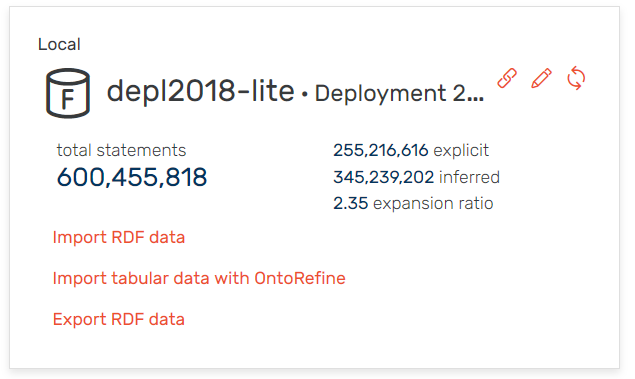
\includegraphics[width=\textwidth]{Figures/active-repository}
\decoRule
\caption[Statements report]{Statements report from the GraphDB workbench.}
\label{fig:statements-report}
\end{figure}

\begin{figure}
\centering
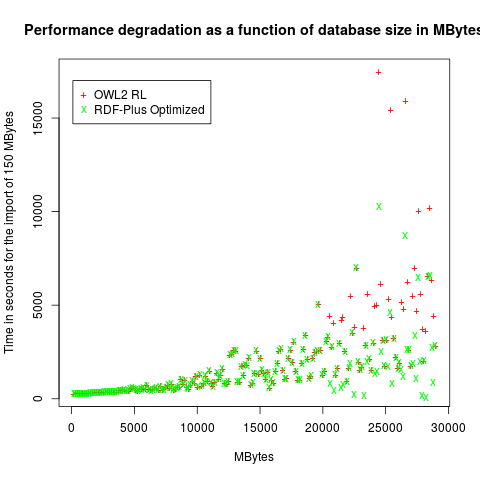
\includegraphics[width=\textwidth]{Figures/performance-degradation-both}
\decoRule
\caption[Performance degradation]{The graph visualizes the time in seconds needed to import a 150 MB big Turtle data file as a function of the database size. The database size is measured by the adding up the size of the data files that have already been imported.}
\label{fig:performance-degradation}
\end{figure}

